\documentclass{article}
\usepackage{amsmath}
\usepackage{amsfonts}
\usepackage[a4paper,width=140mm,top=15mm,bottom=15mm]{geometry}
\usepackage{hyperref}
\usepackage{mathtools}
\usepackage{graphicx}
\graphicspath{ {./figures/} }

\hypersetup{
    colorlinks,
    citecolor=black,
    filecolor=black,
    linkcolor=black,
    urlcolor=black
}

\DeclareUnicodeCharacter{2212}{-}




\title{Esercizi}
\author{Michele Leigheb}
\date{}
\begin{document}
\maketitle
\tableofcontents{}
\section{Complessi}
\begin{itemize}
	\item \(\displaystyle 2^{(a+ib)} = 2^a (\cos(b \ln(2)) + i\sin(b \ln(2))) \)
	\item \(\displaystyle 3^{(a+ib)} = 3^a (\cos(b \ln(3)) + i\sin(b \ln(3))) \)
	\item \(\displaystyle e^{(a+ib)} = e^a (\cos(b)) + i\sin(b) \)
	\item \(\displaystyle \alpha^{(a+ib)} = e^{\alpha} (\cos(b)\ln(\alpha)) + i\sin(b\ln(\alpha)) \)
\end{itemize}



\section{Esercizi}

\section{Esercizio 145 }
 Studiare il sistema \[S:\begin{cases}\overset{\cdot}{x} = \left(\begin{matrix}1 & 1\\-5 & -1\end{matrix}\right) x+ \left(\begin{matrix}0\\1\end{matrix}\right)u\\y = \left(\begin{matrix}0 & 1\end{matrix}\right) x +\left(\begin{matrix}0\end{matrix}\right) u\end{cases}\]\subsection{Studio Risposta Libera}
Si studi la risposta libera di un sistema che ha le seguenti caratteristiche: \[A = \left(\begin{matrix}1 & 1\\-5 & -1\end{matrix}\right)\]
Il determinante di $A-\lambda$ è $ \lambda^{2} + 4 $.

Gli autovalori reali sono $\lambda_i = []$, i complessi sono $\lambda_i = \left[ 2 i, \  - 2 i\right]$.

Gli autovettori associati ai reali sono $ u_i: [   ]$

Gli autovettori associati ai complessi sono $ u_a = \left(\begin{matrix}- \frac{1}{5}\\1\end{matrix}\right), u_b = \left(\begin{matrix}- \frac{2}{5}\\0\end{matrix}\right)$
Da cui posso ricavare le matrici \[U=T^{-1} = \left(\begin{matrix}- \frac{1}{5} & - \frac{2}{5}\\1 & 0\end{matrix}\right), V = T = \left(\begin{matrix}0 & 1\\- \frac{5}{2} & - \frac{1}{2}\end{matrix}\right)\]
Che mi trasformano la matrice in \[ D = TAT^{-1} = \left(\begin{matrix}0 & 2\\-2 & 0\end{matrix}\right) \]
Con $\alpha = 0, \omega =2 $

Da cui posso ricavare: \[ \Phi(t) = e^{At} = T^{-1} e^{Dt} T =  T^{-1} \left(\begin{matrix}\cos{\left(2 t \right)} & \sin{\left(2 t \right)}\\- \sin{\left(2 t \right)} & \cos{\left(2 t \right)}\end{matrix}\right) T\]

\[ = \left(\begin{matrix}\frac{\sin{\left(2 t \right)}}{2} + \cos{\left(2 t \right)} & \frac{\sin{\left(2 t \right)}}{2}\\- \frac{5 \sin{\left(2 t \right)}}{2} & - \frac{\sin{\left(2 t \right)}}{2} + \cos{\left(2 t \right)}\end{matrix}\right) \]\subsubsection{Osservabilità}
 I modi naturali osservabili sono quelli tali che 
\[ C \cdot u_i   \neq 0\]
\subsubsection{Eccitabilità}
 I modi naturali eccitabili sono quelli tali che 
\[v_i' \cdot B \neq 0\]

\subsection{Studio Osservabilità}

Studiamone l’osservabilità. Calcoliamo allora O e troviamo I = ker(O):
\[
 O = \begin{pmatrix}C \\ ... \\ CA^{n-1}  \end{pmatrix} = \left(\begin{matrix}0 & 1\\-5 & -1\end{matrix}\right), |O| = 5 \]
Eccezione 1: O ha rango pieno quindi finisco qui.

\subsection{Studio Raggiungibilità}
Ora per studiare la raggiungibilità degli stati calcolo $R = (B\ AB\ ...\ A^{n-1}B)$: \[ R = \left(\begin{matrix}0 & 1\\1 & -1\end{matrix}\right), |R| = -1 \] 

Vediamo che $rango(R) = 2$ e quindi : \[ \mathfrak{R} = \left[ \left(\begin{matrix}0\\1\end{matrix}\right), \  \left(\begin{matrix}1\\-1\end{matrix}\right)\right] \]

Tutti gli stati che hanno questa struttura sono, allora, raggiungibili. Mettiamo in evidenza questa struttura;
cambiamo base, e vorremmo avere lo stato espresso come $z = Tx$ tale che, se x è uno stato raggiungibile, allora: \[ z_R = T x_R = \begin{pmatrix} \star  \\ 0 \\0\end{pmatrix}\]

E $T^{-1}$ viene \[ T^{-1} = \left(\begin{matrix}0 & 1\\1 & -1\end{matrix}\right) \Longrightarrow T = \left(\begin{matrix}1 & 1\\1 & 0\end{matrix}\right) \]
\[ \overset{\sim}{A} = T A  T^{-1} = \left(\begin{matrix}1 & 1\\1 & 0\end{matrix}\right)\left(\begin{matrix}1 & 1\\-5 & -1\end{matrix}\right)\left(\begin{matrix}0 & 1\\1 & -1\end{matrix}\right) = \left(\begin{matrix}0 & -4\\1 & 0\end{matrix}\right) \]Con le matrici \[ \overset{\sim}{A}_{11} = \left(\begin{matrix}0 & -4\\1 & 0\end{matrix}\right) , \overset{\sim}{A}_{22} = \left(\begin{matrix}\end{matrix}\right)  \]e le matrici \[ \overset{\sim}{B} = TB = \left(\begin{matrix}1\\0\end{matrix}\right)  \]
Ora ne calcoliamo la raggiungibilità: \[ \overset{\sim}{H}(t) = e^{\overset{\sim}{A}t}\overset{\sim}{B} = \begin{pmatrix} e^{\overset{\sim}{A}_{11}t} &  \star \\ 0 & e^{\overset{\sim}{A}_{22}t} \end{pmatrix} \begin{pmatrix} \overset{\sim}{B}_1 \\ 0 \end{pmatrix} = \begin{pmatrix} e^{\overset{\sim}{A_{11}t}}\overset{\sim}{B_1} \\ 0 \end{pmatrix} \]
Quindi infine mi viene che gli autovalori ragg sono $ - 2 i, 2 i,  $ e gli irrag sono $  $
\subsection{Scomposizione di Kalman}
I miei sottospazi di riferimento sono:	\[ \mathfrak{I} = \left[ \right], \mathfrak{R} = \left[ \left(\begin{matrix}0\\1\end{matrix}\right), \  \left(\begin{matrix}1\\-1\end{matrix}\right)\right] \]
La matrice dei vettori di base di I e R è \[ \chi_1 =  \left(\begin{matrix}\end{matrix}\right) \]Ed il determinante è ininfluente.
\paragraph{Per quanto riguarda Chi2:} $ \chi_2 | \chi_2 \oplus \chi_1 = \mathfrak{R} $ è \[ \chi_2 = \left(\begin{matrix}0 & 1\\1 & -1\end{matrix}\right) \]

\paragraph{Per quanto riguarda Chi3:} $ \chi_3 | \chi_3 \oplus \chi_1 = \mathfrak{I} $ è \[ \chi_3 = \left(\begin{matrix}\end{matrix}\right) \]

\paragraph{Per quanto riguarda Chi4:} $ \chi_4 | \chi_1 \oplus \chi_2 \oplus  \chi_3 \oplus \chi_4 = \mathbb{R} $ è \[ \chi_4 = \left(\begin{matrix}\end{matrix}\right) \]
\paragraph{Ora facciamo T inversa:} \[ T^{-1} = (\chi_1\ \chi_2\ \chi_3\ \chi_4\ ) = \left(\begin{matrix}0 & 1\\1 & -1\end{matrix}\right) \]
e quindi \[T = \left(\begin{matrix}1 & 1\\1 & 0\end{matrix}\right)\]
\[ \widetilde{A} = TAT^{-1} = \left(\begin{matrix}-4 & 0\\1 & 1\end{matrix}\right) * T^{-1} = T*\left(\begin{matrix}1 & 0\\-1 & -4\end{matrix}\right) =\left(\begin{matrix}0 & -4\\1 & 0\end{matrix}\right) \]

\[ \widetilde{B} = T B = \left(\begin{matrix}1\\0\end{matrix}\right) \]

\[ \widetilde{C} = C T^{-1} = \left(\begin{matrix}1 & -1\end{matrix}\right) \]
\[Phi(t) = \left(\begin{matrix}\frac{e^{2 i t}}{2} + \frac{e^{- 2 i t}}{2} & i e^{2 i t} - i e^{- 2 i t}\\- \frac{i e^{2 i t}}{4} + \frac{i e^{- 2 i t}}{4} & \frac{e^{2 i t}}{2} + \frac{e^{- 2 i t}}{2}\end{matrix}\right) \]

\subsection{Studio Funzione di trasferimento}

\[ (sI-A) = \left(\begin{matrix}s - 1 & -1\\5 & s + 1\end{matrix}\right), |sI-A| = s^{2} + 4 \]
\[ \Phi(s) = (sI-A)^{-1} = \frac{\left(\begin{matrix}s + 1 & 1\\-5 & s - 1\end{matrix}\right)}{s^{2} + 4} \]

Le funzioni caratteristiche sono \[\begin{array}{rcl}  H(s) & = & \Phi(s)B \\ \Psi(s) & = & C \Phi(s)\\ W(s) & = & C(sI-A)^{-1}B  \end{array} \]

e quindi \[ H(s)  =  \frac{\left(\begin{matrix}1\\s - 1\end{matrix}\right)}{s^{2} + 4} \ \Psi(s) = \frac{\left(\begin{matrix}-5 & s - 1\end{matrix}\right)}{s^{2} + 4} \]
\[ W(s)  =  \frac{\left(\begin{matrix}s - 1\end{matrix}\right)}{s^{2} + 4} = \left(\begin{matrix}\frac{s - 1}{s^{2} + 4}\end{matrix}\right)  \] 
Il grafico di bode è:
\[ W(s) = \frac{s - 1}{s^{2} + 4} \]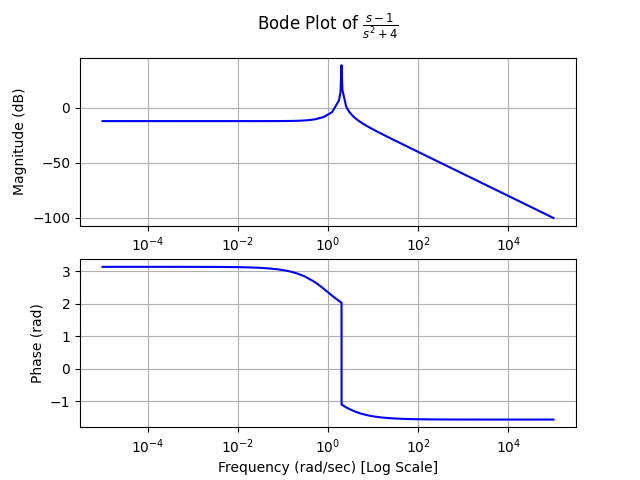
\includegraphics[scale = 0.5]{figures/bode_1189658.png}


Il grafico di Nyquist è:
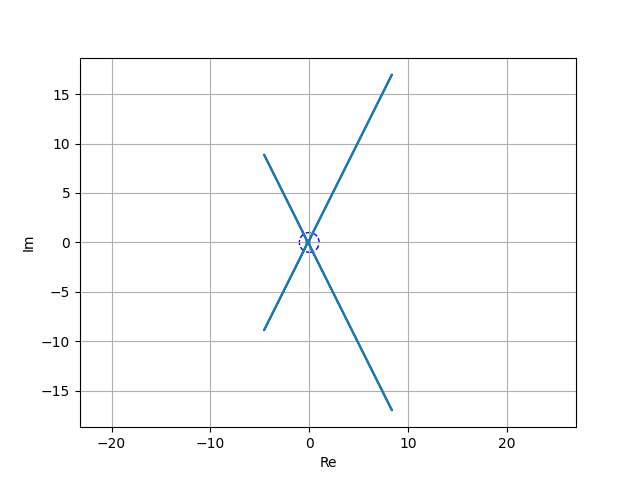
\includegraphics[scale = 0.5]{figures/nyquist_8601915.png}nel tempo continuo è \[ - \frac{\left(\sin{\left(2 t \right)} - 2 \cos{\left(2 t \right)}\right) \theta\left(t\right)}{2} \]
\subsubsection{Vediamo le risposte:} 




























\end{document}
